

\section{In-context learning performance} \label{sec:icl-performance}

%% TODO: Review in-context learning literature here, including CoT, few-shot prompting, and zero-shot prompting. Discuss the differences between these methods and their implications for LLMs' performance in generating mnemonics.
\subsection{Experimental setup}
We systematically compared various in-context learning approaches to understand how different prompting techniques affect mnemonic generation. \Cref{fig:prompting-methods} illustrates the percentage of linguistically grounded mnemonics generated by different prompt formulations.

We used \verb|curator| \citep{BespokeLabBESPOKE2025} with \verb|litellm| orchestration layer to interact with LLM APIs, simpify API calls, manage rate limits, and handle retries.

\subsection{Results}

% \begin{figure}
%   \centering
%   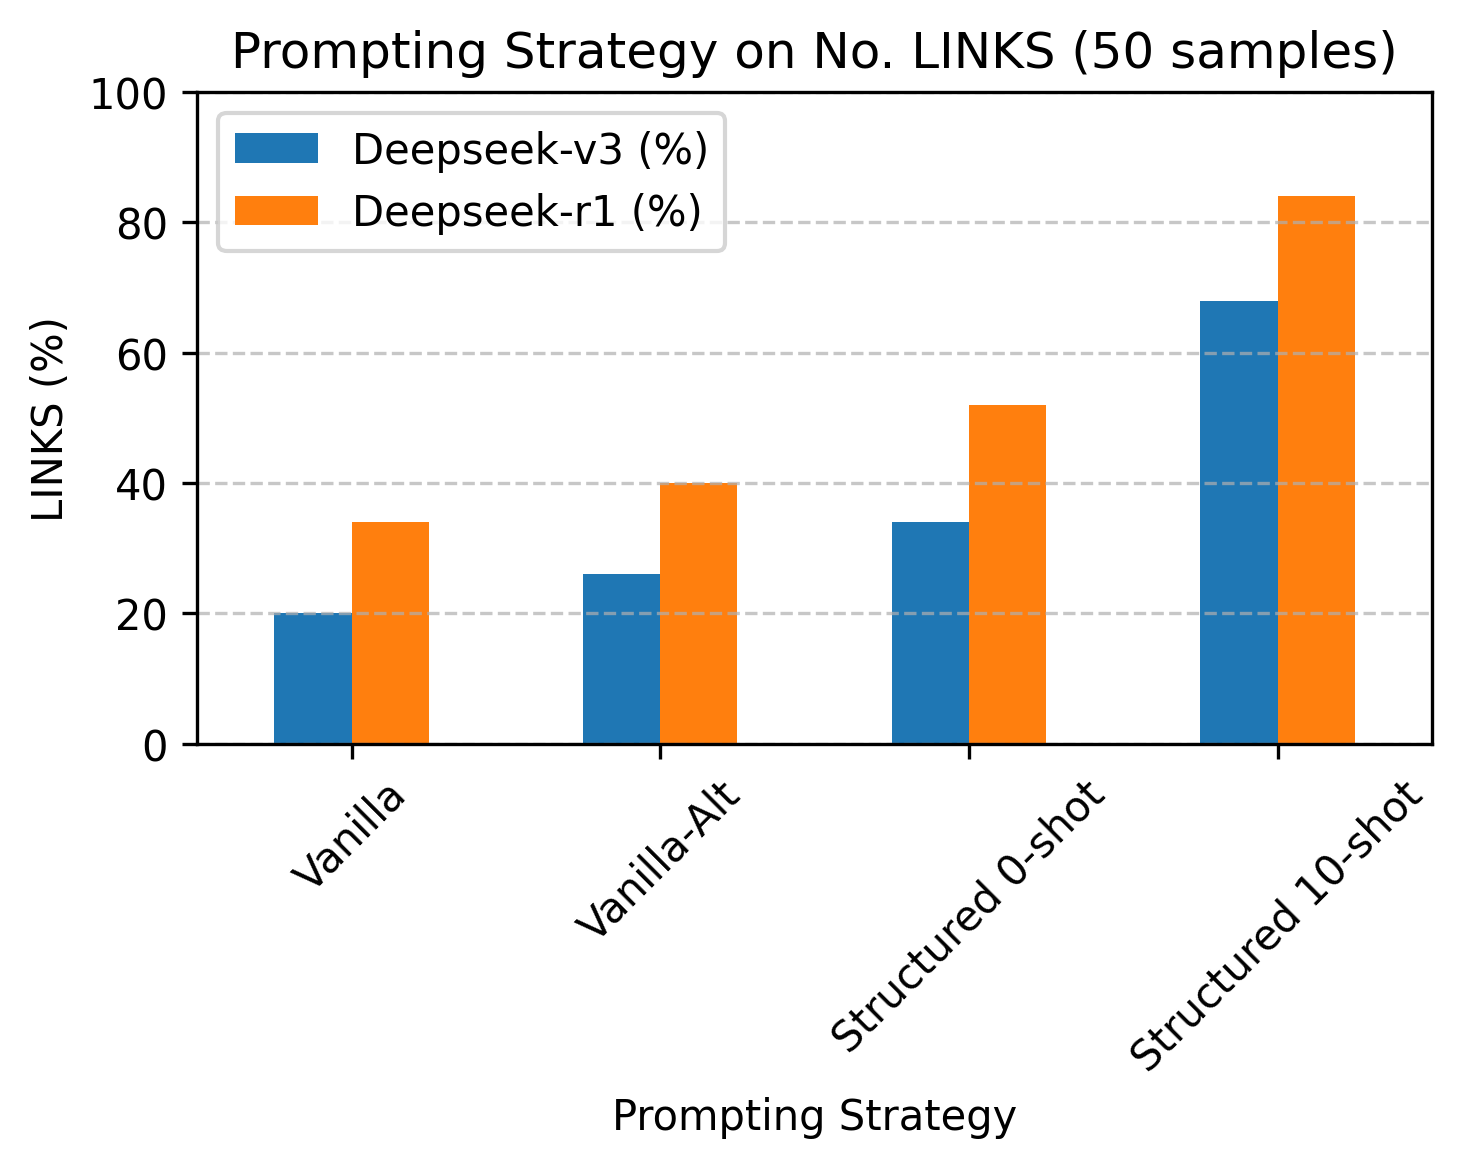
\includegraphics[width=\linewidth]{figures/prompt_comparison.png}
%   \caption{Comparison of prompting methods (see detailed prompt in \Cref{app:prompt-usage}). Y-axis shows percentages of linguistically-grounded mnemonics generated out of 50 requests sent for each prompt type.}
%   \label{fig:prompting-methods}
% % \end{figure}

We observed significant variation in the quality and linguistic grounding of generated mnemonics based solely on prompt formulation. Four distinct prompting strategies were evaluated (see details in \cref{app:prompt-usage})
Vanilla
Reasoning LLMs tend to overthink \citep{xuChainDraftThinking2025}
Good practices: provide decomposed instructions, structured output format, demonstration examples \citep{MishraREFRAMING2022}, and clarify definitions of linguistic features \citep{yinDidYouRead2023}

compress task definition \citep{yinDidYouRead2023},
